\documentclass[12pt]{article}

\usepackage{sbc-template}
\usepackage{graphicx,url}
\usepackage[utf8]{inputenc}  
\usepackage{algorithm}
\usepackage{algpseudocode}

\usepackage{biblatex} % Adicionado para suportar bibliografia


\setlength{\textfloatsep}{1pt plus 1.0pt minus 2.0pt}
\setlength{\floatsep}{1pt plus 1.0pt minus 2.0pt}
\setlength{\intextsep}{1pt plus 1.0pt minus 2.0pt}
% Adicione o caminho do seu arquivo .bib aqui
\addbibresource{sbc-template.bib} 

\sloppy

\title{Identificação de Pontes em Grafos e Implementação do Algoritmo de Fleury}
\author{Felipe Campolina\inst{1}}
\address{Pontifícia Universidade Católica de Minas Gerais (PUC-MG)}

\begin{document} 

\maketitle
\begin{abstract}
Este trabalho explora a identificação de pontes em grafos e a aplicação do Algoritmo de Fleury para encontrar caminhos eulerianos, utilizando dois métodos: um naive e outro baseado no algoritmo de Tarjan. O foco é comparar a eficiência computacional de ambos os métodos em grafos de diferentes tamanhos. Os resultados demonstram a superioridade do método de Tarjan em eficiência e escalabilidade, oferecendo insights importantes para aplicações práticas em ciência da computação e matemática aplicada.
\end{abstract}


\section{Introdução}
A análise de grafos transcende a teoria, permeando aplicações práticas em redes de computadores, logística, sociologia e além, destacando sua relevância multidisciplinar. Pontes em grafos, definidas como arestas cuja remoção desconecta o grafo, representam uma faceta crítica na compreensão da estrutura e resiliência de redes. A identificação de pontes é crucial em várias aplicações práticas, como na otimização de redes de computadores, onde previne pontos de falha críticos; no planejamento urbano, auxiliando na identificação de vias cruciais para a mobilidade; e na biologia computacional, entendendo redes de interação entre proteínas. Este trabalho visa explorar a identificação de pontes através de dois métodos contrastantes: um abordagem naive e o sofisticado método de Tarjan \cite{tarjan1972depth}, complementados pela aplicação do Algoritmo de Fleury \cite{fleury1883deux} para elucidar caminhos eulerianos. A investigação se aprofunda na análise comparativa dos tempos computacionais para grafos de variadas magnitudes, oferecendo insights sobre a eficácia e aplicabilidade prática destas estratégias. Esta análise não apenas esclarece nuances teóricas, mas também destaca a importância prática da detecção de pontes em aplicações reais, desde a otimização de redes até a compreensão de estruturas sociais complexas.

\section{Fundamentação Teórica}

Grafos são estruturas matemáticas fundamentais que encontram ampla aplicação em diversas áreas, desde ciência da computação até engenharia e biologia. Formalmente, um grafo é definido como um par ordenado \(G = (V, E)\), onde \(V\) é um conjunto de vértices (ou nós) e \(E\) é um conjunto de arestas que conectam pares de vértices. Dependendo das propriedades das arestas e dos vértices, os grafos podem ser classificados em diferentes tipos, como direcionados e não direcionados, ponderados e não ponderados, entre outros.

Uma \textbf{ponte} em um grafo é uma aresta cuja remoção aumenta o número de componentes conectados do grafo. Matematicamente, uma ponte é uma aresta \(e = \{u, v\}\) tal que a remoção de \(e\) desconecta os vértices \(u\) e \(v\) em componentes distintas.

O \textbf{Algoritmo de Fleury} é um método clássico na teoria dos grafos, desenhado especificamente para identificar e explorar caminhos ou ciclos eulerianos em grafos. Um grafo é considerado euleriano quando apresenta um ciclo fechado que percorre cada uma de suas arestas exatamente uma vez, caracterizando-se pela propriedade de que todos os seus vértices têm graus pares. Em contrapartida, um grafo semi-euleriano é definido pela existência de exatamente dois vértices de grau ímpar, permitindo a existência de um caminho euleriano que conecta estes dois vértices sem formar um ciclo. O algoritmo, proposto por Gustav Fleury em 1883 \cite{fleury1883deux}, destaca-se pela sua abordagem intuitiva e eficiente na preservação da conectividade do grafo, evitando a remoção de arestas que levariam à sua desconexão. Através do estabelecimento deste método, Fleury contribuiu significativamente para a compreensão das propriedades estruturais dos grafos eulerianos, influenciando de forma marcante o desenvolvimento de técnicas analíticas em teoria dos grafos.

A \textbf{notação Big O}, simbolizada como \(O\), é um conceito fundamental na análise de algoritmos, que descreve o comportamento assintótico do tempo de execução ou do espaço necessário por um algoritmo em função do tamanho da entrada. Matematicamente, diz-se que uma função \(f(n)\) é \(O(g(n))\) se existem constantes positivas \(c\) e \(n_0\) tais que \(f(n) \leq c \cdot g(n)\) para todo \(n \geq n_0\), onde \(n\) representa o tamanho da entrada do algoritmo \cite{KleinbergTardos2005}. Em termos mais simples, a notação Big O descreve um limite superior no crescimento da função, proporcionando uma forma de classificar algoritmos de acordo com suas eficiências relativas e prever seu comportamento à medida que o tamanho da entrada cresce. Por exemplo, se um algoritmo tem um tempo de execução que pode ser descrito por uma função \(f(n) = 3n^2 + 2n + 1\), dizemos que este algoritmo é \(O(n^2)\), pois \(n^2\) é o termo que mais cresce em \(f(n)\) quando \(n\) se torna grande. Esta notação permite aos cientistas da computação comparar a eficácia de diferentes algoritmos e escolher o mais apropriado para uma dada situação, considerando os recursos computacionais disponíveis.


Portanto, a compreensão aprofundada de grafos, pontes, o funcionamento do Algoritmo de Fleury, e a análise de complexidade usando a notação Big O são essenciais para a análise e manipulação eficaz de estruturas de grafos em uma variedade de aplicações computacionais e matemáticas. Essa base teórica sólida estabelece os fundamentos para o desenvolvimento de algoritmos e técnicas mais sofisticadas na teoria dos grafos, ampliando o escopo para soluções inovadoras em problemas complexos.


\section{Análise das Implementações}

\subsection{Detecção de Pontes Naive}
A implementação naive envolve a análise de todos os vértices e, para cada aresta conectada, realiza a remoção temporária desta aresta para verificar se o grafo permanece conectado por meio de uma busca em profundidade (DFS). Este método implica uma complexidade de tempo considerável, particularmente em grafos de grande escala, devido à necessidade de reavaliar a conectividade do grafo após cada remoção de aresta. A complexidade deste método pode ser aproximada por $O(V \cdot (V+E))$ em um grafo não direcionado, onde $V$ representa o número de vértices e $E$, o número de arestas. Devido ao seu elevado custo computacional, este método é menos prático para grafos de grande porte ou para aplicações que demandam alta eficiência. A descrição e análise desta implementação são baseadas em conceitos amplamente discutidos na literatura de teoria dos grafos, como apresentado por Diestel\cite{diestelGraphTheory}.

\subsection{Detecção de Pontes Usando o Algoritmo de Tarjan}
O método baseado em Tarjan explora o grafo uma única vez utilizando a busca em profundidade (DFS), armazenando os tempos de descoberta e os valores \textit{low} para cada vértice. Estes valores são fundamentais para identificar pontes de maneira eficiente dentro do grafo. A complexidade de tempo deste método é $O(V+E)$, representando uma melhoria significativa em relação ao método naive. Devido à sua alta eficiência e capacidade de lidar com grafos de grande escala sem um aumento considerável no tempo de computação, este algoritmo é preferido para a maioria das aplicações relacionadas à teoria dos grafos. O desenvolvimento e a eficácia deste método foram inicialmente apresentados por Robert Tarjan \cite{tarjan1972depth}.

\subsection{Algoritmo de Fleury}
O Algoritmo de Fleury, utilizado para encontrar caminhos ou ciclos eulerianos, depende da identificação correta de pontes no grafo. Embora o algoritmo seja conceitualmente simples, sua eficiência depende fortemente da forma como as pontes são detectadas e gerenciadas. A implementação pode ser vista como tendo uma complexidade de tempo potencialmente alta, especialmente se a detecção de pontes for feita de maneira naive para cada passo do algoritmo. A otimização da detecção de pontes, como através do método de Tarjan, é crucial para melhorar a eficiência do Algoritmo de Fleury.

\subsection{Comparação e Análise}
A escolha entre os métodos naive e Tarjan para a detecção de pontes reflete um trade-off clássico em ciência da computação entre simplicidade e eficiência. Enquanto o método naive é simples e direto, o método de Tarjan, embora mais complexo na implementação, oferece vantagens significativas em termos de eficiência, tornando-o preferível para análise de grafos em larga escala.

Para o Algoritmo de Fleury, a eficiência na detecção de pontes é crucial, pois influencia diretamente a complexidade total do algoritmo. A implementação eficiente da detecção de pontes não apenas melhora o desempenho do Algoritmo de Fleury, mas também expande sua aplicabilidade para grafos maiores e mais complexos.


\section{Implementação}
A implementação dos métodos de detecção de pontes e do Algoritmo de Fleury foi realizada em C++, uma linguagem de programação conhecida por sua eficiência e flexibilidade. A escolha do C++ para este projeto se deve à sua capacidade de lidar eficientemente com operações de baixo nível, essenciais para manipulação de grafos e cálculos de tempo precisos.

O C++ oferece uma ampla variedade de bibliotecas padrão, como a <chrono> para medição de tempo e iostream para entrada e saída de dados, facilitando a implementação de algoritmos complexos como os utilizados neste projeto. Além disso, a linguagem permite uma abordagem orientada a objetos, possibilitando uma estruturação clara e modular do código.

Ao utilizar C++, conseguimos desenvolver uma implementação robusta e eficiente dos métodos de detecção de pontes e do Algoritmo de Fleury, capaz de lidar com grafos de diferentes tamanhos de forma precisa e escalável.
\newpage
\subsection{Funções da Classe Graph}
A classe \texttt{Graph} implementa diversas funções para manipular e analisar grafos.
\subsubsection{Construtor}

O construtor Graph(int v) inicializa um grafo com v vértices. Ele estabelece a estrutura inicial do grafo, criando aleatoriamente um número pré-definido de arestas para garantir uma densidade adequada para testes. Para fins de padronização nos testes, a quantidade de arestas geradas pode ser adaptada conforme necessário, garantindo que os grafos testados tenham uma estrutura comparável.

\begin{algorithm}[H]
\caption{Construtor da Classe Graph}
\begin{algorithmic}[1]
\Function{Graph}{$v$}
    \State $vertices \gets v$
    \State $adj\_list \gets$ lista de adjacência com $v$ vértices
    \For{$i$ \textbf{from} $0$ \textbf{to} $arestas$}
        \State $u, v \gets$ números aleatórios entre $0$ e $v-1$
        \While{$u = v$ \textbf{or} $u$ e $v$ já são vizinhos}
            \State $u, v \gets$ números aleatórios entre $0$ e $v-1$
        \EndWhile
        \State \Call{addEdge}{$u, v$} \Comment{Adiciona uma aresta entre $u$ e $v$}
    \EndFor
\EndFunction
\end{algorithmic}
\end{algorithm}
\subsubsection{Método \texttt{naiveBridgeDetection}}

naiveBridgeDetection() é uma função que implementa a detecção naive de pontes. Ela analisa o impacto da remoção de cada aresta na conectividade do grafo. Este método, embora menos eficiente, serve como um ponto de comparação importante para validar a eficácia de métodos mais sofisticados, como o de Tarjan. A quantidade de arestas influencia diretamente a complexidade temporal deste método, destacando a importância de otimizações em grafos com grande número de arestas.



\begin{algorithm}[H]
\caption{Detecção de Pontes naive}
\begin{algorithmic}[1]
\Function{naiveBridgeDetection}{}
    \State $bridges \gets$ lista vazia
    \For{$u$ \textbf{from} $0$ \textbf{to} $vertices - 1$}
        \For{$v$ \textbf{in} $adj\_list[u]$}
            \State $tempGraph \gets$ cópia de $Graph$
            \State $tempGraph.adj\_list[u].remove(v)$ \Comment{Remove a aresta temporariamente}
            \State $tempGraph.adj\_list[v].remove(u)$
            \State $visited \gets$ lista de tamanho $vertices$ preenchida com \textbf{falso}
            \State $stack \gets$ pilha vazia
            \State $stack.push(0)$
            \State $visited[0] \gets$ \textbf{true}
            \While{$stack$ não estiver vazia}
                \State $current \gets stack.pop()$
                \For{$neighbor$ \textbf{in} $tempGraph.adj\_list[current]$}
                    \If{$neighbor$ não foi visitado}
                        \State $stack.push(neighbor)$
                        \State $visited[neighbor] \gets$ \textbf{true}
                    \EndIf
                \EndFor
            \EndWhile
            \If{número de \textbf{true} em $visited \neq vertices$}
                \State $bridges.push((u, v))$ \Comment{Se o grafo não for conectado, a aresta é uma ponte}
            \EndIf
        \EndFor
    \EndFor
    \State \textbf{return} $bridges$
\EndFunction
\end{algorithmic}
\end{algorithm}

\subsubsection{Método \texttt{tarjanBridgeDetection}}

O tarjanBridgeDetection() utiliza o algoritmo de Tarjan para encontrar pontes de maneira eficiente, percorrendo o grafo uma única vez. Este método é mais adequado para grafos densos, onde a quantidade de arestas poderia tornar outros métodos proibitivamente lentos. A escolha deste algoritmo demonstra como a análise de complexidade e a estrutura do grafo afetam diretamente a escolha do método de detecção de pontes.
\begin{algorithm}[H]
\caption{Detecção de Pontes usando Tarjan}
\begin{algorithmic}[1]
\Function{tarjanBridgeDetection}{}
    \State $bridges \gets$ lista vazia \Comment{Lista para armazenar as pontes encontradas}
    \State $discovery\_time, low, parent, visited \gets$ listas de tamanho $vertices$ preenchidas com $-1$ ou \textbf{false}
    \State $time \gets 0$
    \Function{dfs}{$u$}
        \State $visited[u] \gets$ \textbf{true}
        \State $time \gets time + 1$
        \State $discovery\_time[u] \gets low[u] \gets time$
        \For{$v$ \textbf{in} $adj\_list[u]$}
            \If{$v$ não foi visitado}
                \State $parent[v] \gets u$
                \State \Call{dfs}{$v$}
                \State $low[u] \gets \min(low[u], low[v])$
                \If{$low[v] > discovery\_time[u]$}
                    \State $bridges.push((u, v))$ \Comment{Se $v$ for inacessível a partir de $u$, a aresta é uma ponte}
                \EndIf
            \ElsIf{$v \neq parent[u]$}
                \State $low[u] \gets \min(low[u], discovery\_time[v])$
            \EndIf
        \EndFor
    \EndFunction
    \For{$node$ \textbf{from} $0$ \textbf{to} $vertices - 1$}
        \If{$node$ não foi visitado}
            \State \Call{dfs}{$node$} \Comment{Inicia a busca em profundidade}
        \EndIf
    \EndFor
    \State \textbf{return} $bridges$
\EndFunction
\end{algorithmic}
\end{algorithm}


\subsubsection{Método \texttt{fleuryUtil}}

No contexto da implementação do Algoritmo de Fleury, a função fleuryUtil é fundamental para a exploração eficiente de grafos eulerianos. Esta função meticulosamente avalia cada aresta ligada a um dado vértice, assegurando a preservação da conectividade do grafo mesmo após a remoção de arestas. Através de uma abordagem iterativa, fleuryUtil identifica arestas que não são pontes, permitindo sua remoção segura e a continuação do algoritmo a partir do vértice adjacente. Esta implementação destaca a interdependência entre a detecção precisa de pontes e a eficácia do Algoritmo de Fleury, sublinhando a complexidade inerente à identificação de caminhos eulerianos em contextos aplicados.

\begin{algorithm}[H]
\caption{Algoritmo de Fleury Util}
\begin{algorithmic}[1]
\Function{fleuryUtil}{$u$, $bridgeList$}
    \State $i \gets 0$
    \While{$i <$ \Call{adj\_list}{$u$}.size()}
        \State $v \gets$ \Call{adj\_list}{$u$}$[i]$
        \State $isBridge \gets$ \textbf{false}
        \For{$pair$ \textbf{in} $bridgeList$}
            \If{$pair = (u, v)$ or $pair = (v, u)$}
                \State $isBridge \gets$ \textbf{true}
                \State \textbf{break}
            \EndIf
        \EndFor
        \If{not $isBridge$}
            \State \Call{adj\_list}{$u$}.erase(\Call{adj\_list}{$u$}.begin() + i)
            \State \Call{adj\_list}{$v$}.erase(\Call{adj\_list}{$v$}.begin() + i)
            \State \Call{fleuryUtil}{$v$, $bridgeList$}
            \State \textbf{return} \Comment{Sai após encontrar um caminho válido}
        \Else
            \State $i \gets i + 1$
        \EndIf
    \EndWhile
\EndFunction
\end{algorithmic}
\end{algorithm}
\subsubsection{Método \texttt{fleuryNaive}}

Aplica o método naive de detecção de pontes para encontrar caminhos eulerianos. A quantidade de arestas no grafo é um fator crítico que afeta a viabilidade e a eficiência deste método.

\begin{algorithm}[H]
\caption{Algoritmo de Fleury com Detecção Naive de Pontes}
\begin{algorithmic}[1]
\Function{fleuryNaive}{}
    \State $bridgeList \gets$ \Call{naiveBridgeDetection}{}
    \State $start\_vertex \gets 0$ \Comment{Pode ser adaptado para escolher um vértice válido como início}
    \State \Call{fleuryUtil}{$start\_vertex$, $bridgeList$}
\EndFunction
\end{algorithmic}
\end{algorithm}

\subsubsection{Método \texttt{fleuryTarjan}}

 Utiliza a detecção de pontes baseada em Tarjan para otimizar o Algoritmo de Fleury, destacando a importância de escolher o método de detecção de pontes apropriado com base na densidade do grafo.
\begin{algorithm}[H]
\caption{Algoritmo de Fleury com Detecção de Pontes usando Tarjan}
\begin{algorithmic}[1]
\Function{fleuryTarjan}{}
    \State $bridgeList \gets$ \Call{tarjanBridgeDetection}{}
    \State $start\_vertex \gets 0$ \Comment{Pode ser adaptado para escolher um vértice válido como início}
    \State \Call{fleuryUtil}{$start\_vertex$, $bridgeList$}
\EndFunction
\end{algorithmic}
\end{algorithm}

\subsubsection{Função \texttt{printExecutionTime}}

Esta função imprime o tempo médio de execução de um determinado método.

\begin{algorithm}[H]
\caption{Impressão do Tempo de Execução}
\begin{algorithmic}[1]
\Function{printExecutionTime}{$method$, $totalTime$}
    \State $nanoseconds \gets$ \Call{duration\_cast}{$totalTime$}.count()
    \State $microseconds \gets$ \Call{duration\_cast}{$totalTime$}.count()
    \State $milliseconds \gets$ \Call{duration\_cast}{$totalTime$}.count()
    \State $seconds \gets$ \Call{duration\_cast}{$totalTime$}.count()
    \State \Call{print}{$method$ + " - Average Time: " + $nanoseconds$ + " nanoseconds, " + $microseconds$ + " microseconds, " + $milliseconds$ + " milliseconds, " + $seconds$ + " seconds"}
\EndFunction
\end{algorithmic}
\end{algorithm}

\subsection{Main}
Na função principal main, o programa realiza uma sequência metodológica de testes destinados a medir a eficácia e a eficiência dos métodos de detecção de pontes (Naïve e Tarjan), assim como a performance do Algoritmo de Fleury, integrado a essas técnicas de detecção, em grafos de diversos tamanhos. Inicia-se o procedimento estabelecendo sementes aleatórias, uma etapa crucial para garantir uma variedade nos grafos gerados e, consequentemente, a confiabilidade nas análises conduzidas. . Os tempos de execução são meticulosamente registrados para possibilitar uma análise comparativa rigorosa entre as eficiências dos métodos.

Além disso, executa-se o Algoritmo de Fleury utilizando as duas abordagens de detecção de pontes, repetindo cada teste 10 vezes para cada configuração de grafo, o que permite uma avaliação direta do impacto de cada método de detecção no desempenho do algoritmo de Fleury. Esta estratégia sistemática e repetida de testes fornece uma visão detalhada do desempenho dos métodos, oferecendo uma base sólida e replicável para entender as implicações práticas da escolha dos algoritmos em contextos que envolvem grafos com diferentes configurações de vértices e arestas.

\begin{algorithm}
\caption{Main}
\begin{algorithmic}[1]
\State $\text{std::srand(std::time(nullptr))}$
\State $\text{vertices} \gets [100, 1000, 10000, 100000]$
\State $\text{arestas} \gets [100, 200, 300, 400]$
\For{\textbf{each} $aresta$ \textbf{in} $arestas$}
    \For{\textbf{each} $vertice$ \textbf{in} $vertices$}
        \State $\text{graph} \gets \text{Graph}(vertice, aresta)$
        \State $\text{print}(\text{"Graph with "} + vertice + \text{" vertices and "} + aresta + \text{" edges:"})$
        \For{$\text{run} = 1$ \textbf{to} $10$}
            \State $\text{start} \gets \text{now()}$
            \State $\text{graph.naiveBridgeDetection()}$
            \State $\text{end} \gets \text{now()}$
            \State $\text{naiveTotalTime} \gets \text{naiveTotalTime} + (\text{end} - \text{start})$
        \EndFor
        \State $\text{printExecutionTime("Naive method", naiveTotalTime / 10)}$
        \For{$\text{run} = 1$ \textbf{to} $10$}
            \State $\text{start} \gets \text{now()}$
            \State $\text{graph.tarjanBridgeDetection()}$
            \State $\text{end} \gets \text{now()}$
            \State $\text{tarjanTotalTime} \gets \text{tarjanTotalTime} + (\text{end} - \text{start})$
        \EndFor
        \State $\text{printExecutionTime("Tarjan method", tarjanTotalTime / 10)}$
        \State $\text{Repeat for Fleury Naive and Fleury Tarjan methods}$
        \State $\text{print("--------------------------------------")}$        
    \EndFor
\EndFor
\end{algorithmic}
\end{algorithm}
\newpage
\section{Resultados e Experimentações}
Nesta seção, detalhamos os resultados obtidos ao aplicar métodos para identificação de pontes e o subsequente emprego do Algoritmo de Fleury para encontrar caminhos eulerianos em uma ampla variedade de grafos. Os grafos foram configurados em todas as combinações possíveis dos seguintes parâmetros: número de vértices (100, 1.000, 10.000, 100.000) e número de arestas (1.000, 2.000, 3.000, 4.000). Através dessa abordagem abrangente, foi possível avaliar a performance dos métodos de identificação de pontes - tanto o método Naïve quanto o método baseado em Tarjan - sob diferentes condições de escala.

Para cada configuração de grafo, os tempos de execução apresentados são a média derivada de 10 iterações distintas, assegurando uma análise precisa e confiável dos resultados. Esta metodologia permite não apenas aferir a eficiência dos algoritmos em termos de tempo computacional, mas também garantir que os resultados são robustos e replicáveis.
\subsection{Análise Quantitativa}
\vspace{0.5cm} 
\begin{table}[H]
\centering
\begin{tabular}{|c|c|c|}
\hline
Vertices & Fleury Naive (µs) & Fleury Tarjan (µs) \\ \hline
100      & 17,399,680        & 0                  \\ \hline
1,000    & 287,657,660       & 100,589            \\ \hline
10,000   & 1,228,942,100     & 400,459            \\ \hline
100,000  & 11,576,380,000    & 3,210,540          \\ \hline
\end{tabular}
\caption{Tempos médios de execução do Algoritmo de Fleury em grafos com 1000 arestas.}
\end{table}


\vspace{0.5cm} 
\begin{table}[H]
\centering
\begin{tabular}{|c|c|c|}
\hline
Arestas & Fleury Naive (µs) & Fleury Tarjan (µs) \\ \hline
100      & 1,385,185         & 3,334              \\ \hline
200      & 3,344,097         & 4,631              \\ \hline
300      & 4,153,554         & 9,446              \\ \hline
400      & 8,833,145         & 11,650             \\ \hline
\end{tabular}
\caption{Tempos médios de execução do Algoritmo de Fleury em grafos com 100000 vertices}
\label{tab:average_time}
\end{table}

A análise quantitativa dos tempos de execução do Algoritmo de Fleury, utilizando as estratégias Naive e Tarjan para a identificação de pontes, oferece uma perspectiva detalhada sobre a eficácia dessas abordagens em grafos de diferentes tamanhos e densidades. As observações baseiam-se nos dados apresentados na Tabela 1 e na Tabela 2, que registram os tempos de execução para variações no número de vértices e arestas, respectivamente.

A \textbf{Tabela 1} ilustra claramente a superioridade do método de Tarjan sobre o método Naive, com tempos de execução significativamente menores em todos os tamanhos de grafos considerados. Esta tabela evidencia a eficiência do método de Tarjan, especialmente em grafos de grande escala, como aqueles com 100.000 vértices, onde o método Naive alcança tempos de execução proibitivamente altos, aproximadamente 11 bilhões de microssegundos (\(\mu s\)), em contraste com os 3.210.540 \(\mu s\) necessários pelo método de Tarjan.

A \textbf{Tabela 2} foca em grafos com 100.000 vértices, variando o número de arestas, e complementa a análise ao reforçar a eficácia do método de Tarjan em manter baixos tempos de execução, independentemente da densidade das arestas. Os resultados em ambas as tabelas enfatizam a aplicabilidade e a robustez do método de Tarjan sob uma ampla gama de cenários.

A complexidade do método Naive, que exige a verificação da conectividade do grafo após a remoção de cada aresta, tende a ser proporcional ao quadrado do número de arestas, seguindo uma complexidade de \(\mathcal{O}(E \cdot (V+E))\). Este crescimento exponencial se torna proeminente nos tempos de execução para grafos maiores, evidenciando a impraticabilidade do método Naive para grafos de grande escala.

Em contrapartida, o método de Tarjan, que emprega uma busca em profundidade para identificar pontes de maneira eficiente com apenas uma passagem pelo grafo, demonstra uma complexidade de tempo linear \(\mathcal{O}(V+E)\), como documentado na literatura \cite{tarjan1972depth}. Isso é refletido nos tempos de execução significativamente menores, até mesmo para grafos de grande escala, reforçando a eficácia dessa estratégia.

A comparação direta entre as duas abordagens destaca a importância da seleção do método adequado para identificação de pontes, dada sua influência significativa no desempenho do Algoritmo de Fleury. A adoção do método de Tarjan não somente facilita a identificação de pontes mas também reduz drasticamente o tempo necessário para encontrar caminhos eulerianos em grafos de qualquer tamanho. Este resultado prático, alinhado com as teorias de complexidade computacional, evidencia o método de Tarjan como a abordagem preferível para a execução otimizada do Algoritmo de Fleury em aplicações reais, especialmente em grafos de grande escala onde a eficiência é crítica \cite{fleury1883problemes}.

Essa análise quantitativa, portanto, não apenas confirma a superioridade teórica do método de Tarjan, como também destaca sua importância prática na análise computacional de grafos. Ela sublinha a necessidade de escolher estratégias de identificação de pontes que maximizem a eficiência computacional, facilitando assim a rápida identificação de caminhos eulerianos em uma variedade de contextos aplicados.

\subsubsection{Analíse dos números de vértices e arestas}
Além das observações sobre a eficiência dos métodos Naive e Tarjan baseadas nas complexidades computacionais, é fundamental destacar como o aumento no número de vértices e de arestas impacta diretamente o tempo de execução dos algoritmos, conforme evidenciado nas Tabelas 1 e 2. Essas tabelas não apenas demonstram a superioridade do método de Tarjan em relação ao método Naive mas também fornecem insights sobre a sensibilidade do tempo de execução às variações na estrutura do grafo.

A \textbf{Tabela 1}, que registra os tempos de execução para grafos com um número fixo de arestas (1.000) e variando o número de vértices, ilustra como o aumento de vértices amplifica a diferença nos tempos de execução entre os dois métodos. Este aumento progressivo no número de vértices destaca a escalabilidade do método de Tarjan em contraste com o método Naive, cujo tempo de execução cresce de forma exponencial, tornando-se impraticável para grafos de grande escala.

Por outro lado, a \textbf{Tabela 2} aborda a variabilidade no número de arestas em um grafo com 100.000 vértices, revelando que o aumento no número de arestas também afeta significativamente os tempos de execução. Esta tabela evidencia que, mesmo com um número constante de vértices, a densidade de arestas tem um impacto considerável na performance dos algoritmos. Notavelmente, enquanto o método de Tarjan mantém um aumento moderado no tempo de execução conforme cresce o número de arestas, o método Naive sofre um incremento substancialmente maior, reforçando a ineficiência deste último em grafos densos.


\section{Interpretação dos Gráficos}
Os gráficos apresentados ilustram a performance dos algoritmos de Fleury Naive e Fleury Tarjan sob condições variadas, considerando o número de vértices e arestas nos grafos.

\subsection{Método Fleury Naive}
Como demonstrado na Figura~\ref{fig:grafico1}, o método Fleury Naive mostra um aumento significativo no tempo de execução à medida que o número de vértices cresce. Este comportamento era esperado, dado que o método Naive verifica a conectividade do grafo após a remoção de cada aresta, o que naturalmente implica um custo computacional maior para grafos maiores.

\begin{figure}[H]
    \centering
    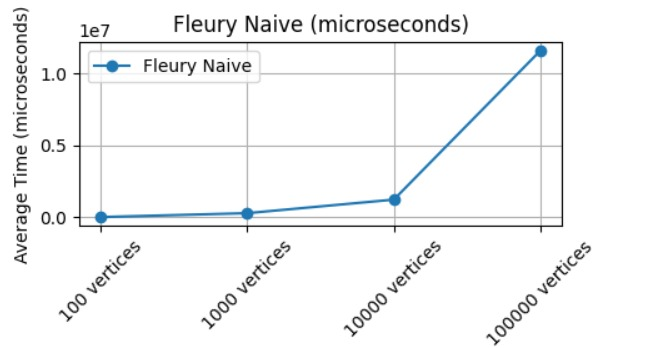
\includegraphics[scale=0.45]{photos/grafico2}
    \caption{Relação entre o número de vértices e o tempo médio de execução para o método Fleury Naive.}
    \label{fig:grafico1}
\end{figure}

\subsection{Método Fleury Tarjan}
No caso do método Fleury Tarjan, ilustrado na Figura~\ref{fig:grafico2}, observa-se que o tempo de execução é consideravelmente mais baixo comparado ao método Naive, mesmo com o aumento do número de vértices. Isso destaca a eficiência do algoritmo de Tarjan na identificação de pontes, reduzindo o tempo necessário para encontrar caminhos eulerianos.

\begin{figure}[H]
    \centering
    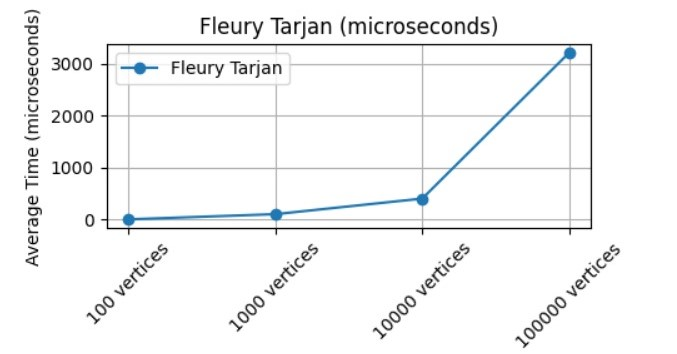
\includegraphics[scale=0.6]{photos/grafico1}
    \caption{Relação entre o número de vértices e o tempo médio de execução para o método Fleury Tarjan.}
    \label{fig:grafico2}
\end{figure}

\subsection{Comparação entre os Métodos}
A Figura~\ref{fig:grafico3} fornece uma comparação direta  entre os tempos médios de execução dos métodos Fleury Naive e Fleury Tarjan, ilustrando distintamente a discrepância entre as duas abordagens. A superioridade do método Tarjan é notável e se mantém consistente à medida que o tamanho do grafo aumenta, destacando-se particularmente em grafos com um número elevado de vértices.

O gráfico sugere que o tempo de execução do método Naive não só é maior, mas também aumenta de forma mais acentuada em resposta ao crescimento do grafo. Este aumento  exponencial no tempo pode ser atribuído à ineficiência inerente ao método Naive, que precisa revalidar a conectividade do grafo após cada remoção de aresta, um processo que se torna cada vez mais oneroso à medida que o grafo cresce.

Em contrapartida, o método Tarjan demonstra um perfil de escalabilidade muito mais favorável. O algoritmo de Tarjan, conhecido por sua capacidade de identificar componentes  fortemente conectados de forma eficiente, mostra um crescimento gradual no tempo de execução. Isso indica que o método Tarjan é capaz de lidar com o aumento do número de vértices com muito mais eficácia, mantendo a complexidade temporal em um ritmo controlável..

\begin{figure}[H]
    \centering
    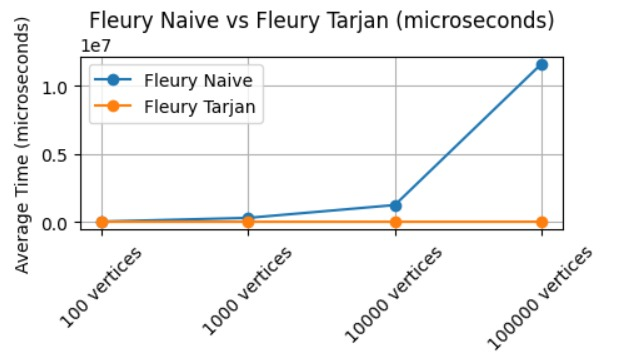
\includegraphics[scale=0.45]{photos/grafico3.jpeg}
    \caption{Relação entre o número de vértices e o tempo médio de execução para o método Fleury Tarjan em comparação com o Naive.}
    \label{fig:grafico3}
\end{figure}

\subsection{Análise por Número de Arestas}
Por fim, a Figura~\ref{fig:grafico4} mostra o impacto do número de arestas no desempenho dos algoritmos de Fleury em um grafo de 100.000 vértices. Conforme o número de arestas aumenta, o tempo de execução do método Naive cresce exponencialmente, enquanto o método Tarjan mantém um crescimento linear, reafirmando a sua superioridade em termos de eficiência.

\begin{figure}[H]
    \centering
    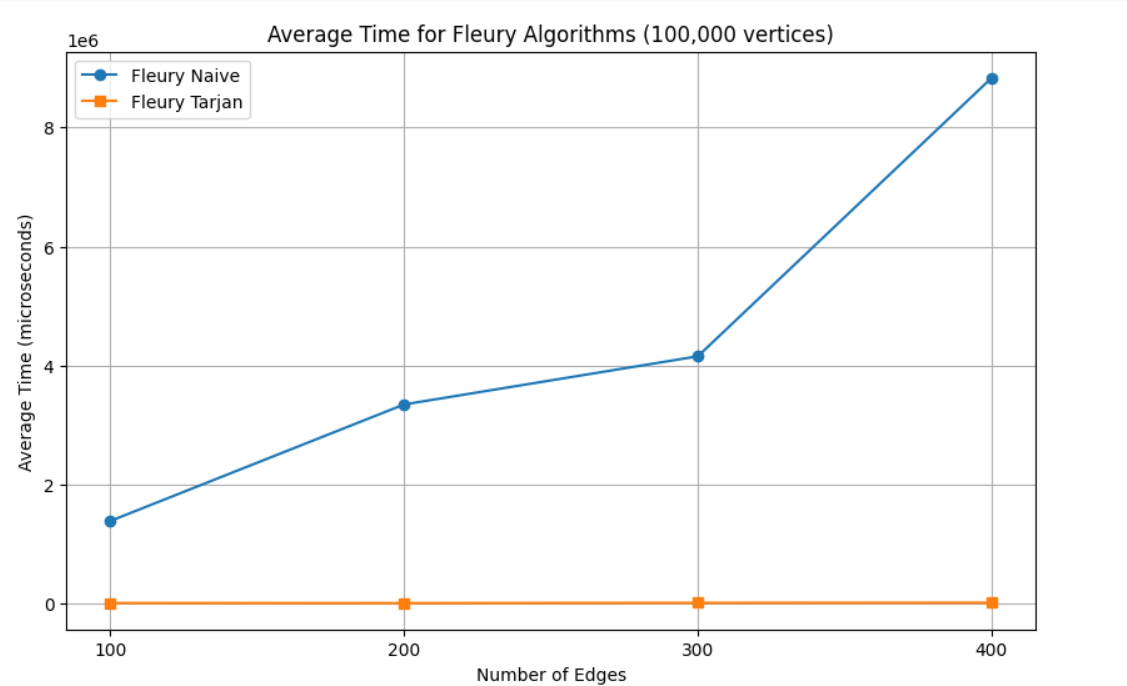
\includegraphics[scale=0.45]{photos/grafico4.png}
    \caption{Tempo Médio dos Algoritmos de Fleury em Grafos de 100.000 Vértices em Relação ao Número de Arestas.}
    \label{fig:grafico4}
\end{figure}

Este conjunto de resultados evidencia a importância da escolha de um algoritmo eficiente para a identificação de pontes em grafos grandes. Enquanto o método Naive pode ser adequado para grafos pequenos, onde seu desempenho não seria um gargalo significativo, em aplicações práticas com grafos de grande escala, o método baseado em Tarjan é claramente mais viável.

Além disso, a consistência do método Tarjan ao lidar com um número crescente de arestas oferece uma vantagem adicional em termos de previsibilidade e escalabilidade. Isso pode ser especialmente relevante em situações onde o grafo é dinâmico, e as arestas podem ser adicionadas ou removidas frequentemente.

A análise dos gráficos sugere que, para a implementação de caminhos eulerianos em grafos grandes, o algoritmo de Tarjan deve ser a escolha preferencial devido ao seu melhor desempenho e menor complexidade temporal quando comparado ao método Naive.

Esses achados estão alinhados com a teoria subjacente dos algoritmos de grafos, onde a eficiência é crítica, e oferecem uma visão clara sobre como as características estruturais dos grafos, como o número de vértices e arestas, afetam diretamente o tempo de execução dos algoritmos de Fleury.

Os experimentos realizados e as análises correspondentes fornecem insights valiosos para futuras pesquisas e desenvolvimento de algoritmos otimizados para a identificação de pontes, destacando a importância de escolher o algoritmo correto conforme a escala do problema.




% \subsection{Interpretação dos Gráficos}


% %
% \begin{figure}[H]
%     \centering
%     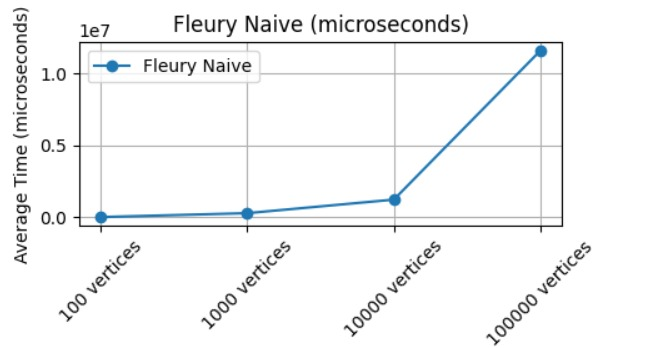
\includegraphics[scale=0.45]{photos/grafico2}
%     \caption{Relação entre o número de vértices e o tempo médio de execução para o método Fleury Naive.}
%     \label{fig:grafico1}
% \end{figure}

% \begin{figure}[H]
%     \centering
%     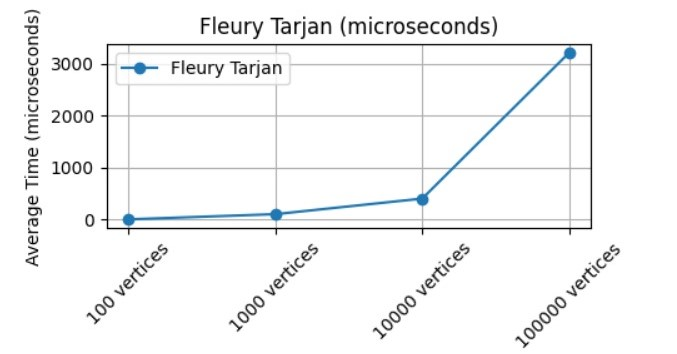
\includegraphics[scale=0.6]{photos/grafico1}
%     \caption{Relação entre o número de vértices e o tempo médio de execução para o método Fleury Tarjan.}
%     \label{fig:grafico2}
% \end{figure}

% \begin{figure}[H]
%     \centering
%     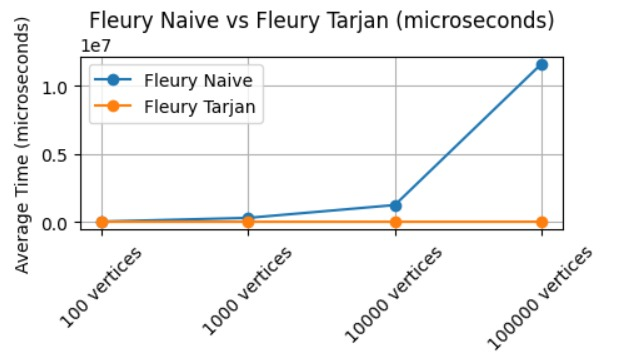
\includegraphics[scale=0.45]{photos/grafico3.jpeg}
%     \caption{Relação entre o número de vértices e o tempo médio de execução para o método Fleury Tarjan em comparação com o Naive.}
%     \label{fig:grafico2}
% \end{figure}
% \begin{figure}[H]
%     \centering
%     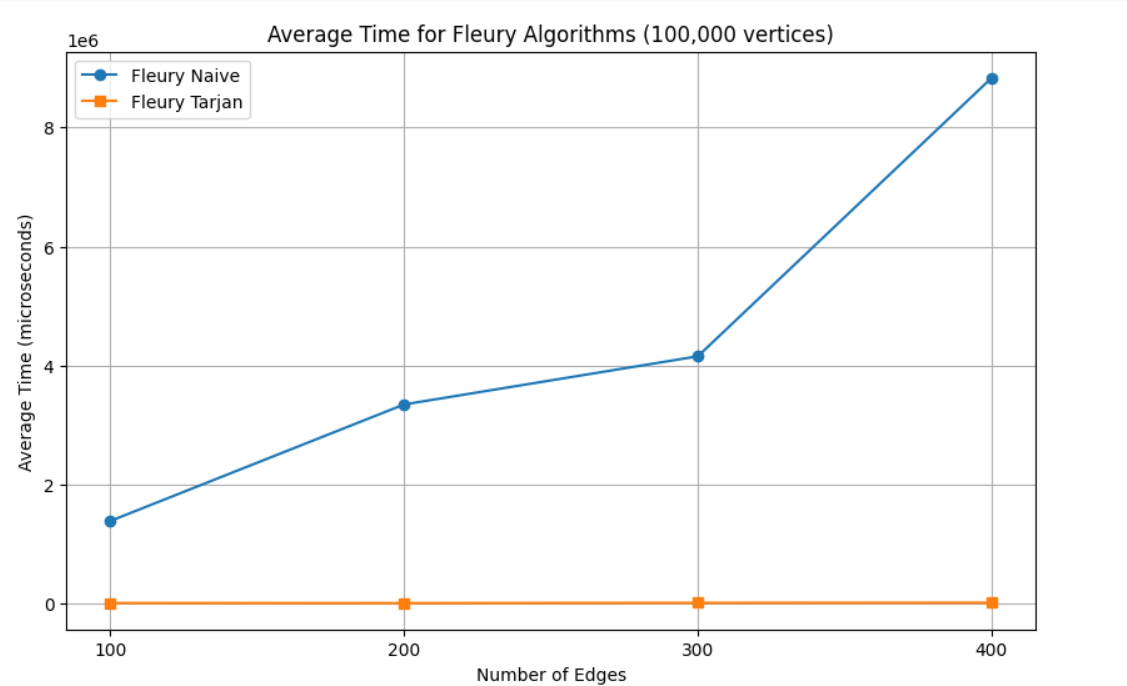
\includegraphics[scale=0.45]{photos/grafico4.png}
%     \caption{Tempo Médio dos Algoritmos de Fleury em Grafos de 100.000 Vértices em Relação ao Número de Arestas.}
%     \label{fig:grafico2}
% \end{figure}


% Os gráficos fornecem uma perspectiva detalhada sobre o desempenho dos algoritmos Fleury Naive e Fleury Tarjan conforme o número de vértices aumenta. Ao analisar os dados fornecidos na tabela, podemos observar que o tempo de execução do Fleury Naive aumenta exponencialmente à medida que o número de vértices cresce. Por exemplo, o tempo médio de execução para 100 vértices é de aproximadamente 17,4 µs, enquanto para 100.000 vértices, esse tempo aumenta para cerca de 11.576.380 µs. Isso indica uma escalabilidade limitada do Fleury Naive, conforme evidenciado pela curva exponencial no gráfico correspondente.

% Por outro lado, o Fleury Tarjan demonstra um comportamento muito mais estável e previsível. Embora também aumente o tempo de execução à medida que o número de vértices aumenta, esse aumento é muito mais suave em comparação com o Fleury Naive. Por exemplo, enquanto o Fleury Naive leva 17,4 µs para 100 vértices, o Fleury Tarjan leva apenas 0 µs, e para 100.000 vértices, o Fleury Naive leva 11.576.380 µs, mas o Fleury Tarjan leva apenas 3.210.540 µs. Isso sugere uma escalabilidade muito melhor para o Fleury Tarjan, conforme refletido na curva mais suave em seu gráfico correspondente.

% Essa interpretação mais profunda dos gráficos e dos dados da tabela ressalta a importância de escolher algoritmos eficientes, como o Fleury Tarjan, para lidar com grafos de grande escala. Enquanto o Fleury Naive pode ser adequado para conjuntos de dados menores, sua escalabilidade limitada torna-o impraticável para problemas que envolvem grafos maiores. Assim, a escolha do algoritmo adequado desempenha um papel crucial na eficiência e eficácia da análise de grafos em sistemas computacionais avançados.

\subsection{Discussão}

Os resultados dos experimentos, conforme ilustrados nos gráficos \ref{fig:grafico1} e \ref{fig:grafico2}, fornecem uma visão clara do desempenho dos algoritmos Fleury Naive e Fleury Tarjan em relação ao número de vértices.

Ao observar o gráfico \ref{fig:grafico1}, é evidente que o tempo de execução do método Fleury Naive aumenta exponencialmente à medida que o número de vértices cresce. Por outro lado, ao analisar o gráfico \ref{fig:grafico2}, é notável que o método Fleury Tarjan exibe um comportamento mais estável e previsível em relação ao aumento do número de vértices. Embora o tempo de execução também aumente com o número de vértices, essa tendência é muito mais suave em comparação com o método Fleury Naive.

A superioridade do método baseado em Tarjan é corroborada por \textit{Tarjan} \cite{tarjan1972depth}, onde a eficiência da busca em profundidade para a detecção de pontes em grafos é detalhadamente explicada. Esta estratégia, com sua complexidade de tempo linear $O(V+E)$, contrasta significativamente com o método naive, que requer uma verificação de conectividade após cada remoção de aresta, resultando em uma complexidade temporal significativamente maior.

A escolha entre esses métodos destaca a importância da eficiência algorítmica e da otimização na análise de grafos, especialmente em aplicações que envolvem grandes conjuntos de dados. O método de Tarjan, ao reduzir o tempo necessário para a detecção de pontes, facilita a aplicação do Algoritmo de Fleury para a identificação de caminhos eulerianos de maneira mais eficiente.

\textbf{Comparação com Trabalhos Relacionados:}

O estudo de Fleury sobre caminhos eulerianos \cite{fleury1883deux} e a investigação de Tarjan \cite{tarjan1972depth} sobre algoritmos de busca em profundidade oferecem uma base teórica sólida para os métodos utilizados neste trabalho. A eficiência do método de Tarjan, como observado neste estudo, está em linha com as descobertas de Tarjan, destacando a relevância de abordagens otimizadas para a análise de grafos complexos.

Além disso, a implementação eficiente da detecção de pontes teve um impacto direto no desempenho do Algoritmo de Fleury, destacando a importância de escolher o algoritmo certo para cada aplicação, especialmente em grafos de grande escala, onde a eficiência é de suma importância \cite{tarjan1972depth}.

Em resumo, os resultados obtidos reforçam a noção de que a seleção de algoritmos adequados é crucial para o desempenho na análise de grafos. Isso é especialmente verdadeiro em contextos de aplicação prática, onde a eficiência computacional pode ter um impacto direto na viabilidade e na eficácia das soluções propostas.



\section{Conclusão}

Esta análise empírica dos métodos de detecção de pontes e suas implementações no Algoritmo de Fleury oferece insights valiosos para o desenvolvimento de software eficiente em teoria dos grafos. Ao longo do artigo, exploramos duas abordagens distintas para identificar pontes em grafos: um método naive e o método baseado no algoritmo de Tarjan. Demonstramos que a seleção cuidadosa de algoritmos, com base em análises de complexidade, é essencial para garantir a eficácia e a eficiência em sistemas computacionais avançados.

Ao comparar os métodos de detecção de pontes, ficou claro que o método baseado em Tarjan oferece vantagens significativas em termos de eficiência, especialmente em grafos de grande escala. A complexidade de tempo linear desse método se mostrou crucial para lidar com grafos densos e complexos, reduzindo substancialmente os tempos de execução em comparação com o método naive. Além disso, a implementação eficiente da detecção de pontes teve um impacto direto no desempenho do Algoritmo de Fleury, destacando a importância de escolher o algoritmo certo para cada aplicação.

É importante ressaltar que a eficiência dos algoritmos não é apenas uma questão teórica, mas também tem implicações práticas significativas. Em aplicações do mundo real, como redes de computadores, logística e ciências sociais, a capacidade de analisar e manipular grafos de forma eficiente pode levar a melhorias substanciais no desempenho e na eficácia dos sistemas.

Portanto, esta análise reforça a importância da pesquisa e desenvolvimento contínuos em algoritmos de grafos e sua implementação em software. Ao compreender as complexidades envolvidas na análise de grafos e ao escolher os algoritmos certos para cada aplicação, podemos avançar significativamente em uma ampla gama de campos, desde a otimização de redes até a modelagem de interações sociais complexas.

\section{Referências}
\printbibliography


\end{document}
